\section{Реализация}


\subsection{Конфигурация}
\begin{frame}{Конфигурация среды тестирования производительности}
	Тесты проводились на следующей аппаратной конфигурации:
	\begin{itemize}
		\item 8 процессоров Intel Xeon E5-2580 2.4 ГГц;
		\item 64 Гб оперативной памяти.
	\end{itemize}
	Операционная система: Ubuntu 16.04. Для тестирования был установлен Docker версии 18.04.0-ce.
	
	\vspace{1em}
	\centering
	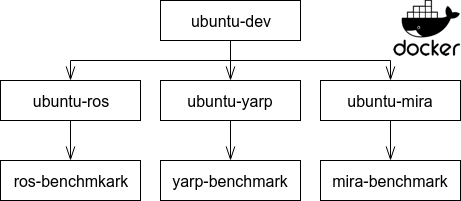
\includegraphics[scale=.5]{img/dockers.png}
\end{frame}

\subsection{Бенчмарки}
\begin{frame}{Требования к инструменту измерения производительности}
	Измеряемые характеристики:
	\begin{itemize}
		\item Задержка передачи сообщений между зулами (нс)
		\item Полоса пропускания канала коммуникации (б/с)
	\end{itemize}
	Требования к инструменту:
	\begin{itemize}
		\item Точность вычисления:
		\begin{itemize}
			\item Высокоточные часы \texttt{std::chrono}
			\item Такты процессора \texttt{asm rdtsc}
		\end{itemize}
		\item Сериализация результатов в файл
		\item Возможность приостанавливать учет времени
		\item Итеративность выполнения тестов
	\end{itemize}

	Решения:
	\begin{itemize}
		\item Google Benchmark framework
		\item Собственная библиотека Benchmark gripper (причина: MIRA)
	\end{itemize}
\end{frame}

\begin{frame}{Benchmark Gripper: сценарии использования и диаграмма состояний}
	\begin{columns}[onlytextwidth]
		\begin{column}{0.49\textwidth}
			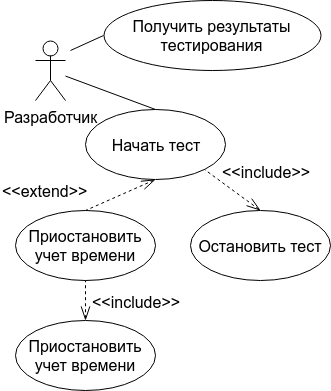
\includegraphics[width=\textwidth]{img/uc.png}
		\end{column}
		\begin{column}{0.49\textwidth}
			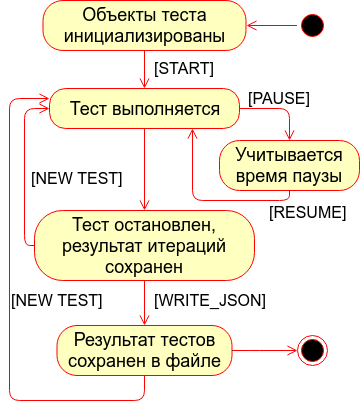
\includegraphics[width=\textwidth]{img/sm.png}
		\end{column}
	\end{columns}
\end{frame}

\begin{frame}{Benchmark Gripper: диаграмма классов}
\centering
	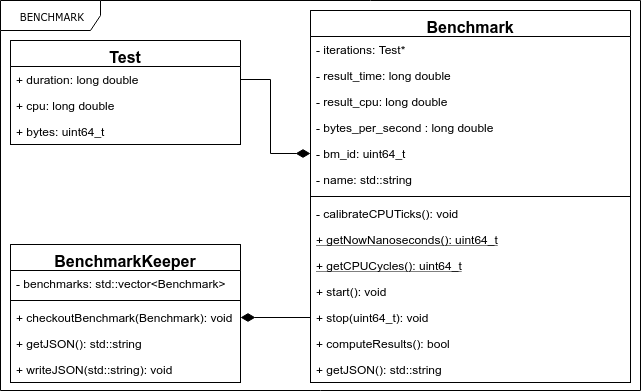
\includegraphics[scale=.46]{img/class.png}
\end{frame}

\begin{frame}{Benchmark Gripper: преимущества и недостатки}
	Преимущества:
	\begin{itemize}
		\item не требуется предварительная компиляция
		\item интерфейс основан на макросах
		\item высокая точность
		\item сериализация результатов совместимая с Google Benchmark
	\end{itemize}
	Недостатки:
	\begin{itemize}
		\item скудный по-сравнению с Google benchmark функционал
		\item длительное исполнение тестов
	\end{itemize}
\end{frame}


\subsection{Анализатор}
\begin{frame}{Анализатор результатов - Merger.py}
	\begin{columns}[onlytextwidth]
		\hspace{-0.5cm}
		\begin{column}{0.45\textwidth}
			\begin{itemize}
				\item Принимает на вход:
				\begin{itemize}
					\item множество результатов в формате json
					\item файлы конфигурации
				\end{itemize}
				\item Статистически обрабатывает результаты
				\item Результат - файл rmarkdown
			\end{itemize}
		\end{column}
		\begin{column}{0.6\textwidth}
			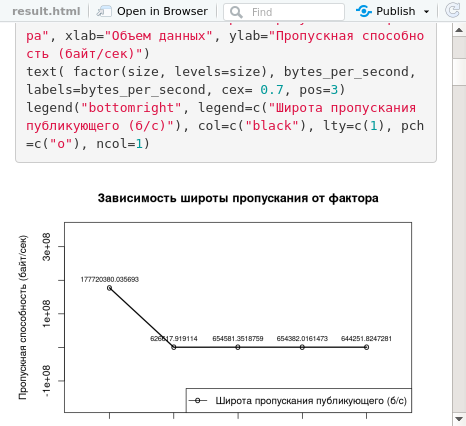
\includegraphics[width=\textwidth]{img/tmp.png}
		\end{column}
	\end{columns}
	
\end{frame}

\subsection{Система}
\begin{frame}{Система тестирования производительности}
	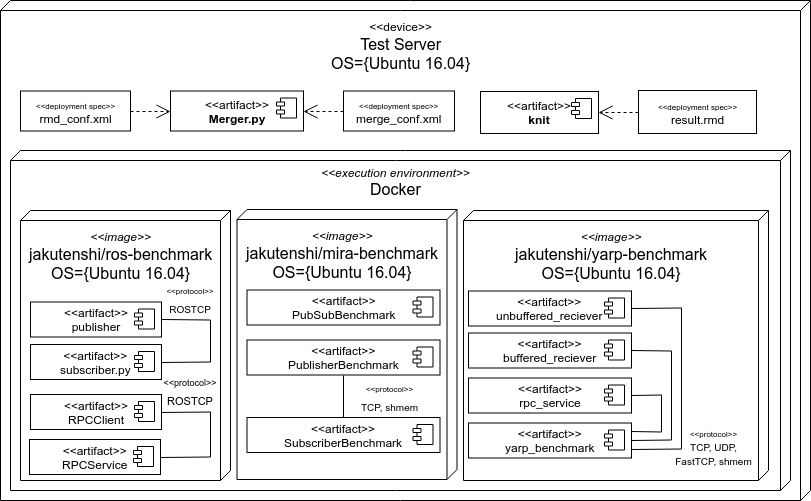
\includegraphics[scale=.37]{img/deploy.png}
\end{frame}